\chapter{Pendahuluan}
\label{chap:intro}
   
\section{Latar Belakang}
\label{sec:label}
Zaman sekarang ada banyak masalah-masalah terkait transportasi yang sudah mulai mempengaruhi hampir semua orang, seperti pemanasan global akibat gas emisi kendaraan, kemacetan di mana-mana, dan bagi pemilik kendaraan bermotor, semakin meningginya harga BBM (bahan bakar minyak). Upaya dari pemerintah untuk menyelesaikan atau meringankan masalah-masalah ini adalah dengan mendorong masyarakat untuk menggunakan sarana transportasi publik. Di Indonesia ada beberapa jenis transportasi umum, sama seperti di negara-negara lain, seperti kereta api, bus, taksi, tetapi satu jenis transportasi umum belum tentu ada di negara-negara lain adalah angkutan kota, atau sering kali disingkat menjadi ``angkot''.

Angkot (dapat dilihat di Gambar \ref{fig:intro-angkot}) merupakan sebuah unit transportasi umum yang metode operasinya menyerupai bus, hanya saja penumpang angkot dapat meminta pengemudinya untuk turun di mana saja, selama lokasinya masih berada di dalam rute yang sudah ditentukan untuk unit angkot tersebut. Hal ini membuat rute angkot esensial untuk diketahui, karena pengetahuan mengenai lokasi mana saja yang akan dilewati unit-unit angkot yang dinaiki dapat menghemat waktu perjalanan\textemdash apabila lokasi yang ingin dituju dilewati oleh unit angkot tersebut, tetapi bukan merupakan pemberhentian akhirnya, penumpangnya dapat langsung meminta pengendara angkot untuk berhenti di lokasi tersebut. Sistem ini menimbulkan dua masalah lain. Pertama, untuk pergi dari suatu lokasi ke lokasi lain, pengguna juga harus mengetahui unit-unit angkot mana saja yang harus dinaiki. Kedua, untuk mengefektifkan waktu perjalanan dengan angkot, penggunanya juga harus mengetahui persis lokasi-lokasi mana saja yang dilewati oleh unit angkot yang dinaiki. 

\begin{figure}[h]
    \centering
    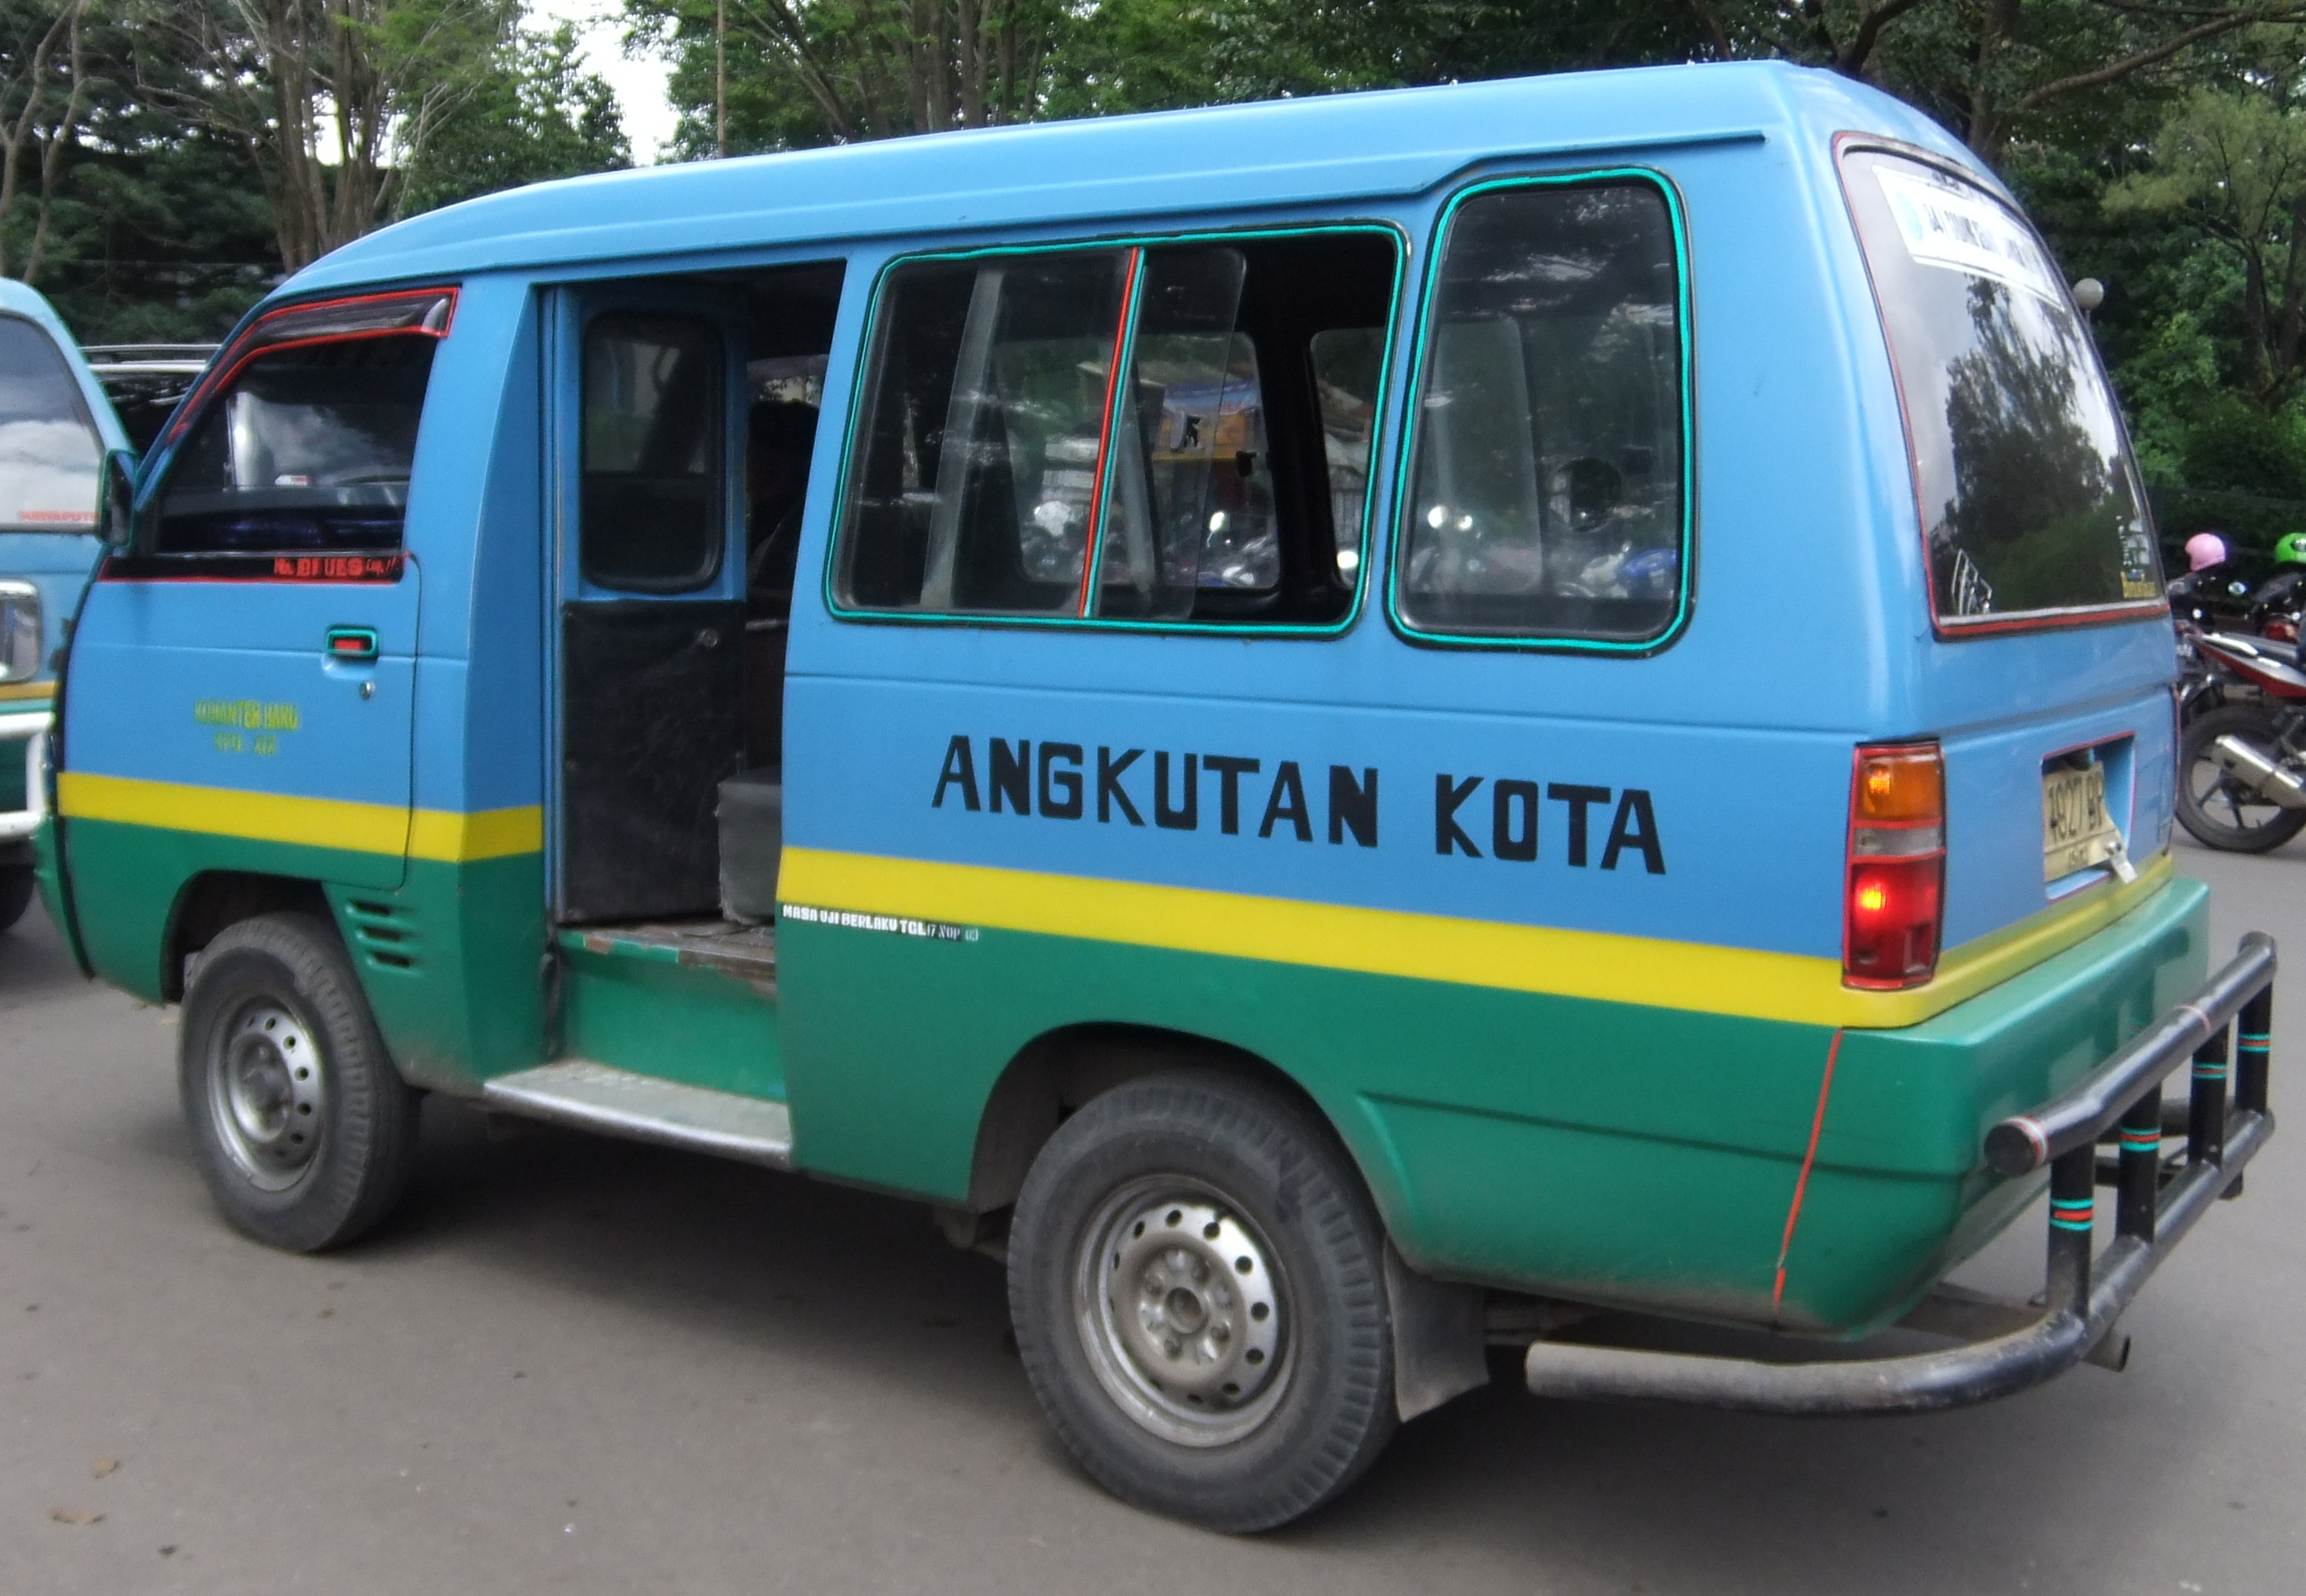
\includegraphics[width=0.5\linewidth]{intro-angkot}
    \caption[Unit angkot]{Unit mobil angkutan kota (angkot).}
    \label{fig:intro-angkot}
\end{figure}

Masalah inilah yang merupakan salah satu tujuan dari Project KIRI. Project KIRI\footnote{\href{https://projectkiri.id}{https://projectkiri.id}} (akan disingkat sebagai KIRI dalam dokumen ini) adalah sebuah \websoftware\xspace yang dibuat untuk membantu penggunanya, baik masyarakat maupun turis, dalam menggunakan angkot. Cara KIRI mempermudah penggunaan angkot adalah dengan menunjukkan rute yang akan ditempuh, beserta langkah-langkah yang harus dilakukan oleh pengguna yang ingin berpergian dari satu titik ke titik lain, mulai dari seberapa jauh pengguna harus berjalan untuk menaiki angkot yang bersangkutan, di mana pengguna harus naik atau turun, seberapa jauh lagi pengguna harus berjalan sampai ke titik tujuan, dan seberapa lama estimasi waktu perjalanan yang akan ditempuh\textemdash semua di halaman \textit{web} dari KIRI, yang dapat dilihat di Gambar \ref{fig:kiri-page}. Walaupun begitu, dalam kasus-kasus tertentu KIRI memiliki berbagai keterbatasan, misalnya pencarian lokasi tidak akurat, atau rute angkot tidak berhasil ditemukan (walaupun bisa jadi ada rute angkot yang cukup dekat dengan lokasi awal dan tujuan), dsb.

\begin{figure}[ht]
    \centering
    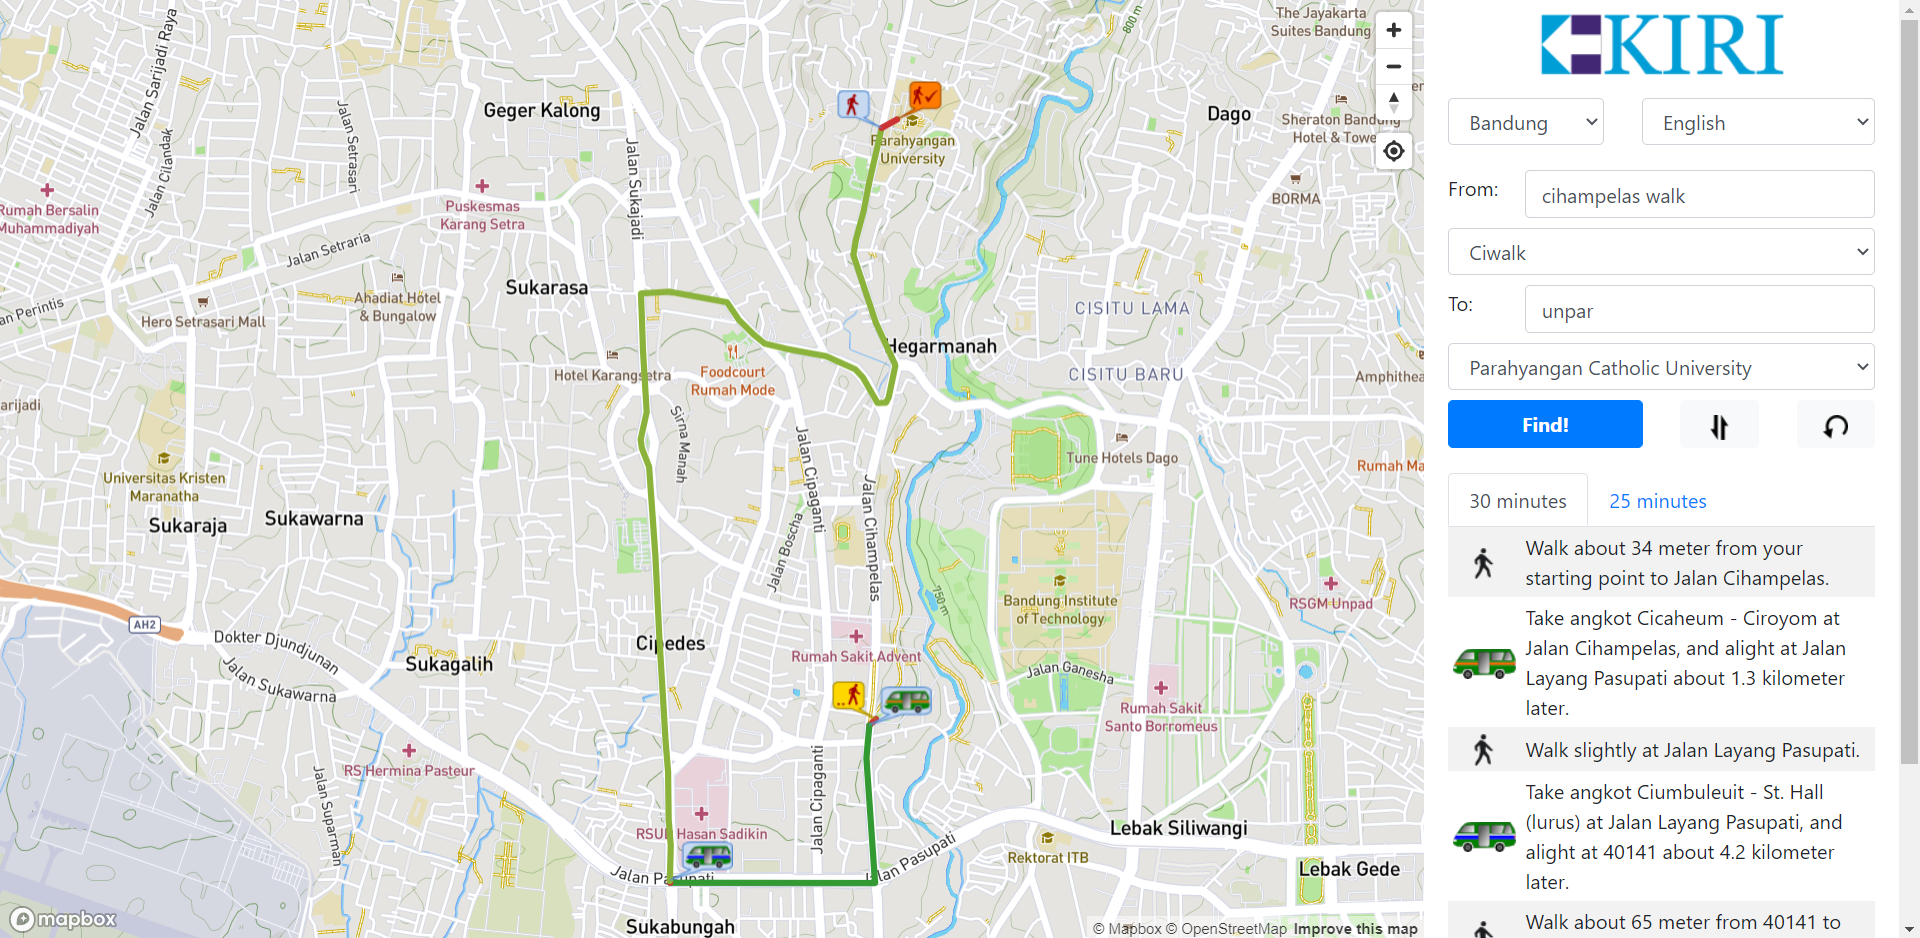
\includegraphics[width=0.875\linewidth]{projectkiri-example}
    \caption[Tampilan halaman web KIRI]{Tampilan halaman web KIRI, yang menunjukkan rute dari Cihampelas Walk ke Universitas Katolik Parahyangan.}
    \label{fig:kiri-page}
\end{figure}

Pada saat penulisan skripsi ini, KIRI hanya dapat diakses langsung melalui halaman \textit{web}-nya, di mana aplikasi ini memiliki banyak bantuan elemen-elemen grafis, yang menjadikannya sebuah aplikasi berbasis antarmuka pengguna grafis (\gui /GUI). GUI ini hanya merupakan satu dari dua jenis antarmuka perangkat lunak, dengan jenis antarmuka satu lagi berupa antarmuka baris perintah (\cli /CLI). \textit{Command line interface} adalah sebuah antarmuka yang berupa sebuah \textit{window} yang memuat teks berupa perintah-perintah,\footnote{\href{https://ubuntu.com/tutorials/command-line-for-beginners\#3-opening-a-terminal}{https://ubuntu.com/tutorials/command-line-for-beginners\#3-opening-a-terminal}} yang menerima masukan dari pengguna dan  menjalankannya \cite{marsh:2010:fatfreeintrotocommandline}. Perintah-perintah ini hanya berupa gabungan dari teks and simbol-simbol berupa karakter. Singkatnya, tipe perangkat lunak ini bukan merupakan tipe yang paling indah untuk dilihat oleh para pengguna, tetapi jika digunakan dengan tepat, maka \mbox{jenis} \mbox{perangkat} lunak ini bisa menyuruh komputer untuk melakukan banyak sekali perintah-perintah dengan sangat cepat dan sangat efektif \cite{shottsjr:2019:linuxcommandline}.

Walaupun tipe antarmuka CLI muncul lebih awal dari GUI, sampai sekarang juga masih banyak perangkat-perangkat lunak yang memiliki versi CLI, atau bahkan hanya berbentuk CLI. Ada beberapa alasan CLI masih dipakai di perangkat-perangkat lunak modern, seperti \cite{matthew:2007:beginninglinuxprogramming}:

\begin{itemize}
	\item penggunaannya lebih cepat dan sederhana,
	\item selalu kompatibel di berbagai sistem operasi, bahkan di instalasi-instalasi yang paling mendasar, dan
	\item kesederhanaannya membuat CLI lebih ideal digunakan untuk tugas-tugas di mana kemudahan konfigurasi lebih penting dari efisiensi dibandingkan GUI.
\end{itemize}

Selain aplikasi \textit{web}-nya sendiri, KIRI juga memiliki antarmuka pemrograman aplikasi (\api /API) yang dapat digunakan untuk tujuan pengembangan perangkat lunak\footnote{\href{https://projectkiri.id}{https://projectkiri.id}}. API ini merupakan sebuah antarmuka logikal ke perangkat lunak serta menyembunyikan detail-detail internal implementasinya. Dalam kata lain, API menyediakan sebuah abstraksi untuk sebuah masalah serta mendiktekan bagaimana klien/penggunanya harus berinteraksi dengan komponen perangkat lunak yang menyelesaikan masalah tersebut. Secara esensi, API akan mendefinisikan bagian-bagian yang dapat digunakan ulang, yang memungkinkan potongan-potongan fungsi modular yang dapat langsung diimplementasikan ke perangkat-perangkat lunak lainnya \cite{reddy:2011:apidesigncpp}. Khusus untuk kasus ini, API KIRI dapat digunakan dengan mengirimkan permintaan GET, dan nantinya akan mengeluarkan keluaran berupa objek JSON\footnote{\href{https://github.com/projectkiri/Tirtayasa/wiki/KIRI-API-v2}{https://github.com/projectkiri/Tirtayasa/wiki/KIRI-API-v2}}.

Pada skripsi ini akan dibuat sebuah perangkat lunak berupa perkakas \cl\xspace (\cl\xspace\textit{tool}) yang dapat menjalankan fungsi-fungsi API dari KIRI. Perangkat lunak ini, seperti jenisnya, akan dibuat murni sebagai perkakas yang dijalankan dari \cl (Terminal, cmd, PowerShell, dll.). Keseluruhan dari perangkat lunak ini akan dibangun dalam bahasa C\textemdash bahasa C dipakai karena penggunaan bahasa ini memungkinkan pengaturan manual besar memori sistem yang dipakai oleh perkakas \cite{raymond:2003:artofunixprogramming} (karena perkakas termasuk perangkat lunak yang ringan, maka memori maksimum yang boleh digunakan dapat diatur sekecil mungkin.) Selain itu, perkakas ini juga akan menggunakan bantuan fungsi bahasa C, yaitu getopt untuk penerimaan opsi-opsi masukan, serta \textit{library-library} tambahan, seperti libcurl untuk proses transfer data, cJSON untuk mem-\textit{parse} keluaran API, dan CMake untuk kompatibilitas antar sistem operasi. Bagaimana dan kapan persisnya modul-modul ini akan digunakan di dalam perkakas yang akan dibuat akan dibahas di bagian perancangan. Terakhir, perkakas akan memiliki fitur-fitur perkakas \cl\xspace pada umumnya, seperti halaman/mode bantuan, serta akan memiliki kemampuan integrasi dengan perkakas-perkakas \cl\xspace lainnya, dalam arti bahwa keluaran dari perkakas ini akan bisa digunakan sebagai masukan untuk perkakas-perkakas \cl\xspace lainnya yang sudah ada, seperti \textit{pipeline} (\verb|>|) atau \verb|grep|.

\section{Rumusan Masalah}
\label{sec:rumusan}
Rumusan masalah yang akan dibahas dalam skripsi ini adalah sebagai berikut:
\begin{enumerate}
	\item Bagaimana membangun perkakas \textit{command line} yang dapat mengimplementasikan fitur-fitur API KIRI dalam bahasa C?
	\item Bagaimana integrasi perkakas \textit{command line} KIRI dapat dilakukan dengan perkakas-perkakas \textit{command line} lainnya?
\end{enumerate}

\section{Tujuan}
\label{sec:tujuan}
Tujuan dari skripsi ini adalah sebagai berikut:
\begin{enumerate}
	\item Membangun perkakas \textit{command line} yang dapat mengimplementasikan fitur-fitur API KIRI dalam bahasa C.
	\item Melakukan integrasi perkakas \textit{command line} KIRI dengan perkakas-perkakas \textit{command line} lainnya.
\end{enumerate}
\vspace{-0.5em} % Prevent section widow
\section{Batasan Masalah}
\label{sec:batasan}
% Batasan masalah dalam skripsi ini adalah sebagai berikut:
% \begin{enumerate}
Perkakas yang dibuat hanya akan menyelesaikan batasan yang berhubungan langsung dengan format keluaran (kesalahan terjemahan) yang sudah sejak awal terdapat dalam KIRI. Batasan-batasan lain yang tidak berhubungan dengan format keluaran (lokasi tidak terdeteksi, rute tidak berhasil ditemukan, dsb.) akan ditulis di keluaran perkakas apa adanya.
% \end{enumerate}

\section{Metodologi}
\label{sec:metlit}
Metodologi yang akan diikuti dalam skripsi ini adalah sebagai berikut:
	\begin{enumerate}
		\item Melakukan studi dan eksplorasi terhadap fungsi-fungsi yang dimiliki perangkat lunak KIRI serta cara implementasi API KIRI.
		\item Melakukan analisis dan desain perangkat lunak yang akan dibangun.
	    \item Melakukan studi dan eksplorasi terhadap seluruh kemungkinan \textit{library-library} yang memenuhi spesifikasi dalam pembuatan perangkat lunak, berdasarkan analisis dan desain yang telah dilakukan sebelumnya.
		\item Melakukan analisis kebutuhan fitur-fitur perangkat lunak dan melakukan eksplorasi \textit{library} yang dapat digunakan dan memenuhi spesifikasi dalam pembuatan perangkat lunak.
		\item Membangun perangkat lunak berdasarkan rancangan yang sudah dibuat, dengan mengimplementasikan seluruh modul dan \textit{library} yang telah ditentukan di tahap sebelumnya dalam bahasa C.
		\item Melakukan pengujian fungsional, perbaikan \textit{bug}, serta rekomendasi perbaikan berdasarkan pengujian yang sudah dilakukan, jika diperlukan.
		\item Menyelesaikan pembuatan dokumen-dokumen yang berkaitan, seperti dokumen skripsi dan dokumentasi perangkat lunak.
	\end{enumerate}

\section{Sistematika Pembahasan}
\label{sec:sispem}
Setiap bab dalam skripsi ini mengikuti sistematika yang terdiri atas poin-poin sebagai berikut:
\begin{enumerate}
	\item \textbf{Bab 1}: Pendahuluan \\
	Bab ini berisi latar belakang, rumusan masalah, tujuan, batasan masalah, metodologi \mbox{penelitian}, dan sistematika pembahasan.
	\item \textbf{Bab 2}: Dasar Teori \\
	Bab ini berisi pembahasan-pembahasan teoretis mengenai aspek-aspek yang akan dirujuk di dalam skripsi ini, seperti \cl, bahasa C, dan juga KIRI.
	\item \textbf{Bab 3}: Analisis \\
	Bab ini berisi analisis perkakas-perkakas sejenis, analisis API KIRI, serta analisis fitur-fitur perkakas yang akan dibuat.
	\item \textbf{Bab 4}: Perancangan \\
	Bab ini berisi pembahasan mengenai rancangan cara kerja tiap-tiap fitur serta fungsi-fungsi dalam kode perkakas yang akan dibuat.
	\item \textbf{Bab 5}: Implementasi dan Pengujian \\
	Bab ini berisi dua bagian utama, yaitu:
	
	\begin{itemize}
		\item Implementasi \\
		Bagian ini meliputi struktur kelas dan penjelasan tiap-tiap fungsi di dalamnya.
		\item Pengujian \\
		Bagian ini meliputi cara instalasi, cara menggunakan perkakas, serta pengujian fungsional terhadap fitur-fitur dari perkakas yang telah dibuat.
	\end{itemize}
	
	\item \textbf{Bab 6}: Kesimpulan dan Saran \\
	Bab ini berisi kesimpulan hasil pembuatan perangkat lunak dan saran-saran terhadap hasil perangkat lunak yang diberikan selama pengerjaan skripsi.
\end{enumerate}